%
%  Chris Thoma
%
\documentclass[12pt,fullpage]{article}
\usepackage{fullpage}
\usepackage{psfrag}                                          % LaTeX graphics tool
\usepackage{pslatex}                                         % avoids the default cmr font
\usepackage{graphicx}                                        % graphics package 
\usepackage{epsfig}                                          % figures
\usepackage{hyperref}
\usepackage{color}

\begin{document}

\noindent
{\bf Logistic distribution} (from \color{blue}\url{http://www.math.wm.edu/~leemis/chart/UDR/UDR.html}\color{black})

\noindent
The shorthand $X \sim {\rm logistic}(\lambda, \kappa)$ is used to indicate that the
random variable $X$ has the logistic distribution with parameters $\lambda$ and $\kappa$.
A logistic random variable $X$ with positive scale parameter~$\lambda$ and positive shape parameter $\kappa$ 
has probability density function 
$$
f(x) = \frac{\lambda ^ \kappa \kappa \kern 0.08 em e ^ {\kappa \kern 0.04 em x}}{(1 + (\lambda e ^ x) ^ \kappa) ^ 2} \qquad \qquad -\infty < x < \infty.
$$
The probability density function with three different parameter settings is illustrated below.
\begin{figure}[h!]
\begin{center}
\psfrag{lab1}{$\lambda \kern -0.08 em = \kern -0.08 em  .05,\, \kappa \kern -0.08 em  = \kern -0.08 em  3$}
\psfrag{lab2}{$\lambda \kern -0.08 em  = \kern -0.08 em  .001,\, \kappa \kern -0.08 em  = \kern -0.08 em  .75$}
\psfrag{lab3}{$\lambda \kern -0.08 em  = \kern -0.08 em  .005,\, \kappa \kern -0.08 em  = \kern -0.08 em  1.5$}
\psfrag{labx}{$x$}
\psfrag{labf}{$f(x)$}
\includegraphics[width=3.2in]{LogisticPlot.ps}
\end{center}
\end{figure}\\
The cumulative distribution function on the support of $X$ is 
$$
F(x) = P(X \le x) = \frac{\lambda^\kappa e ^{\kappa\kern 0.04 em x}}{1+\lambda^\kappa e^x} \qquad \qquad -\infty < x < \infty. 
$$
The survivor function on the support of $X$ is
$$
S(x) = P(X \ge x) =
\frac{1  + \lambda^\kappa e^{\kern 0.04 em x} - \lambda^\kappa e^{\kern 0.04 em x \kern 0.04 em \kappa}}
{1+\lambda^\kappa e^{\kern 0.04 em x}}\qquad \qquad -\infty < x < \infty.
$$
The hazard function on the support of $X$ is
$$
h(x) = \frac{f(x)}{S(x)} =
\frac{\kappa e^{\kern 0.04 em \kappa \kern 0.04em x}(\lambda^\kappa + \lambda^{2\kappa}e^{\kern 0.04 em x})}
{
(1 + (\lambda e ^ x) ^ \kappa) ^ 2
(1  + \lambda^\kappa e^{\kern 0.04 em x} - \lambda^\kappa e^{\kern 0.04 em x \kern 0.04 em \kappa})
}
\qquad \qquad -\infty < x < \infty.
$$
The inverse distribution function of $X$ is
$$
F ^ {-1}(u) = - \frac{1}{\kappa} \ln \left(\frac{u}{1-u} \right) - \ln \lambda \qquad \qquad 0 < u < 1.
$$
The moment generating function of $X$ is
$$
M(t) = E\left[ e ^ {tX} \right] =
\displaystyle \int_{-\infty} ^\infty \frac{\lambda^\kappa \kappa e^{\kern 0.04 em x(t+\kappa)}}{(1+ \lambda^\kappa e^{\kern 0.04 em x\kern 0.04 em \kappa})^2} \, dx.
$$
The characteristic function of $X$ is
$$
\phi(t) = E\left[ e ^ {itX} \right] =
\displaystyle \int_{-\infty} ^\infty \frac{\lambda^\kappa \kappa e^{\kern 0.04 emx(it+\kappa)}}{(1+ \lambda^\kappa e^{\kern 0.04 em x \kern 0.04 em \kappa})^2} \, dx.
$$
The population mean and variance are
$$
E[X] = -\ln \lambda \qquad \qquad 
V[X] = \frac{\pi^2}{3 \kappa^2}. 
$$
The population skewness and kurtosis of $X$ are more complicated expressions. \\
%   For $X_1, \, X_2, \, \ldots , \, X_n$ mutually independent logistic($\lambda$) random variables,
%   the maximum likelihood estimator for $\lambda$ is
%   $$
%   \hat \lambda = \frac{n}{\sum_{i\,=\,1}^n X_i}.
%   $$

\noindent
{\bf APPL verification:}
The APPL statements
\begin{verbatim}
X := LogisticRV(kappa, lambda);
CDF(X);
SF(X);
HF(X);
IDF(X);
MGF(X);
Mean(X);
Variance(X);
\end{verbatim}
verify the cumulative distribution, survivor function, hazard function,  inverse distribution function, moment generating function, population mean, and variance.
\end{document}
